\documentclass[a4paper,oneside,12pt]{extreport}

\usepackage{mmap}
\usepackage[T2A]{fontenc}
\usepackage[utf8]{inputenc}
\usepackage[english,russian]{babel}


% Текст отчёта следует печатать, соблюдая следующие размеры полей:
% левое — 30 мм, правое — 15 мм, верхнее и нижнее — 20 мм.
\usepackage[left=20mm, right=15mm, top=15mm, bottom=15mm]{geometry}

% \setlength{\parindent}{1.25cm} % Абзацный отступ

\usepackage{setspace}
%\onehalfspacing % Полуторный интервал

\frenchspacing % Равномерные пробелы
\usepackage{indentfirst} % Красная строка

\usepackage{microtype}
\sloppy

\usepackage{titlesec}
\titlespacing*{\chapter}{0pt}{-30pt}{8pt}
\titlespacing*{\section}{\parindent}{*4}{*4}
\titlespacing*{\subsection}{\parindent}{*4}{*4}
\titleformat{\chapter}{\LARGE\bfseries}{\thechapter}{20pt}{\LARGE\bfseries}
\titleformat{\section}{\Large\bfseries}{\thesection}{40pt}{\Large\bfseries}

\usepackage{graphicx}
\usepackage{caption}

\usepackage[unicode,pdftex]{hyperref}
\hypersetup{hidelinks}

%% title begin
\usepackage{wrapfig}

\makeatletter
	\def\vhrulefill#1{\leavevmode\leaders\hrule\@height#1\hfill \kern\z@}
\makeatother
%% title end

%% begin code
\usepackage{listings}
\usepackage{xcolor}

\lstset{
	basicstyle=\footnotesize\ttfamily,
	breakatwhitespace=true,
	breaklines=true,
	commentstyle=\color{gray},
	frame=single,
	keywordstyle=\color{blue},
	stringstyle=\color{red},
	tabsize=8
}

\lstdefinestyle{lispinline}{
	frame=none,
	language=Lisp
}

\newcommand{\code}[1]{\texttt{#1}}
%% end code

%% begin theorem
\usepackage{amsthm}

\makeatletter
\newtheoremstyle{indented}
	{}% measure of space to leave above the theorem
	{}% measure of space to leave below the theorem
	{}% name of font to use in the body of the theorem
	{\parindent}% measure of space to indent
	{\bfseries}% name of head font
	{.}% punctuation between head and body
	{ }% space after theorem head; " " = normal interword space
	{}% header specification (empty for default)
\makeatother

\theoremstyle{indented}

\newtheorem{definition}{Определение}[section]
\newtheorem{example}{Пример}[section]
\newtheorem{theorem}{Теорема}[section]
\newtheorem{task}{Задание}

\makeatletter
\DeclareRobustCommand\bfseriesitshape{%
	\not@math@alphabet\itshapebfseries\relax
	\fontseries\bfdefault
	\fontshape\itdefault
	\selectfont
}
\makeatother

\DeclareTextFontCommand{\textbfit}{\bfseriesitshape}
\DeclareTextFontCommand{\define}{\bfseriesitshape}
%% end theorem

%% begin columns
\usepackage{etoolbox,refcount}
\usepackage{multicol}

\newcounter{countitems}
\newcounter{nextitemizecount}
\newcommand{\setupcountitems}{%
	\stepcounter{nextitemizecount}%
	\setcounter{countitems}{0}%
	\preto\item{\stepcounter{countitems}}%
}
\makeatletter
\newcommand{\computecountitems}{%
	\edef\@currentlabel{\number\c@countitems}%
	\label{countitems@\number\numexpr\value{nextitemizecount}-1\relax}%
}
\newcommand{\nextitemizecount}{%
	\getrefnumber{countitems@\number\c@nextitemizecount}%
}
\newcommand{\previtemizecount}{%
	\getrefnumber{countitems@\number\numexpr\value{nextitemizecount}-1\relax}%
}
\makeatother
\newenvironment{AutoMultiColItemize}{%
	\ifnumcomp{\nextitemizecount}{>}{3}{\begin{multicols}{2}}{}%
		\setupcountitems\begin{itemize}}%
		{\end{itemize}%
		\unskip\computecountitems\ifnumcomp{\previtemizecount}{>}{3}{\end{multicols}}{}}
\makeatother
\newenvironment{AutoMultiColEnumerate}{%
	\ifnumcomp{\nextitemizecount}{>}{3}{\begin{multicols}{2}}{}%
		\setupcountitems\begin{enumerate}}%
		{\end{enumerate}%
		\unskip\computecountitems\ifnumcomp{\previtemizecount}{>}{3}{\end{multicols}}{}}
%% end columns

	
\usepackage{amsmath}

\begin{document}

\begin{titlepage}
	{\large % 14pt instead of 12pt
	\onehalfspacing
	\centering

	\begin{wrapfigure}[7]{l}{0.14\linewidth}
		\vspace{3mm}
		\hspace{-10mm}
		
\includegraphics[width=\linewidth]{img/b_logo}
		% \includegraphics[width=0.93\linewidth]{inc/img/bmstu-logo}
	\end{wrapfigure}
	{\singlespacing \footnotesize \bfseries Министерство науки и высшего образования Российской Федерации\\Федеральное государственное бюджетное образовательное учреждение\\высшего образования\\<<Московский государственный технический университет\\имени Н.~Э.~Баумана\\ (национальный исследовательский университет)>>\\(МГТУ им. Н.~Э.~Баумана)\\}

	\vspace{-2.2mm}
	\vhrulefill{0.9mm}\\
	\vspace{-7.5mm}
	\vhrulefill{0.2mm}\\
	\vspace{2mm}

	{\doublespacing \small \raggedright ФАКУЛЬТЕТ \hspace{5mm} \underline{«Информатика и системы управления»}\\
	КАФЕДРА \hspace{10mm} \underline{«Программное обеспечение ЭВМ и информационные технологии»}\\}

	\vspace{20mm}

	\begin{center}
		\noindent\begin{minipage}{1.2\textwidth}\centering
			\textbf{ОТЧЕТ ПО ЛАБОРАТОРНОЙ РАБОТЕ №4}\newline
			\textbf{По курсу: "Моделирование"}\newline\newline\newline
		\end{minipage}
	\end{center}

	\vspace{20mm}

	\noindent ~~Тема \underline{~~~~~Программно-алгоритмическая реализация моделей~~~~~~~~~~~~~~~~~~~~~}\newline
	\underline{~~~~~~~~~~~~~~на основе дифференциальных уравнений в~~~~~~~~~~~~~~~~~~~~~~~~~~~~~~~~~}\newline
	\underline{~~~~~~~частных производных с краевыми условиями II и III рода.~~~~~~~~~~~~~~~~~~}\newline
	\noindent ~~Группа \underline{~~~~~~~~~~~~~~~~~~~~~~~~~~~~~~~~~~~ИУ7-63Б~~~~~~~~~~~~~~~~~~~~~~~~~~~~~~~~~~~~~~~~~~~~~~~~~}\newline
	\noindent ~~Студент \underline{~~~~~~~~~~~~~~~~~~~~~~~~~~~~Сукочева А.~~~~~~~~~~~~~~~~~~~~~~~~~~~~~~~~~~~~~~~~~~~~~~~~~~}\newline
	\noindent ~~Преподаватель \underline{~~~~~~~~~~~~~~~~~Градов В.М.~~~~~~~~~~~~~~~~~~~~~~~~~~~~~~~~~~~~~~~~~~~~~~~~~~~}\newline


	\begin{center}
		\vfill
		Москва~---~\the\year
		~г.
	\end{center}
	}



\end{titlepage}

\setcounter{page}{2}

\section{Постановка задачи}
\textbf{Цель работы}. 
Получение навыков разработки алгоритмов решения краевой задачи при
реализации моделей, построенных на ОДУ второго порядка.

\subsection{Исходные данные}

Задана математическая модель:

\begin{equation*}
	\frac{d}{dx}(\lambda(T)\frac{dT}{dx}) - 4 \cdot k(T) \cdot n_{p}^2 \cdot \sigma \cdot (T^4 - T_{0}^4) = 0
\end{equation*}\\

Краевые условия:

\begin{equation*}
	\begin{cases} x = 0, -\lambda(T(0))\frac{dT}{dx} = F_{0}.
	\\ x = l, -\lambda(T(l))\frac{dT}{dx} = \alpha(T(l) - T_{0})
	\end{cases}
\end{equation*}\\

Функции $\lambda(T)$ и $k(T)$ заданы таблицей.\\

\begin{figure}[ht!]
	\centering{
		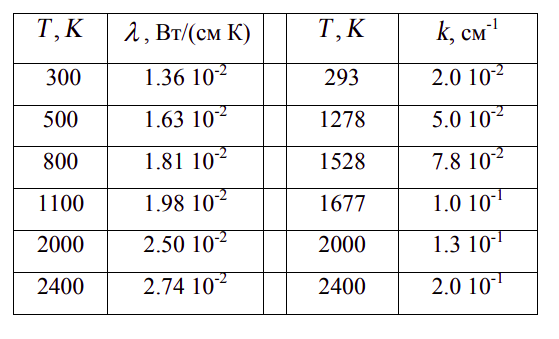
\includegraphics[width=0.6\textwidth]{img/table.png}
		\caption{Таблица функций $\lambda(T)$ и $k(T)$ } }
\end{figure}

Заданы начальные параметры:\\
\indent $n_p$ = 1.4 - коэффициент преломления\\
\indent $l$ = 0.2 см - толщина слоя\\
\indent $T_{0}$ = 300К - температура окружающей среды\\
\indent $\sigma$ = 5.668 $\cdot 10^{-12}$ Вт / ($cm^2 \cdot K^4$) - постоянная Стефана - Больцмана\\
\indent $F_{0}$ = 100 Вт / $cm^2$ - поток тепла\\
\indent $\alpha$ = 0.05 Вт / ($cm^2 \cdot K$) - коэффициент теплоотдачи\\

Выход из итераций организовать по температуре и по балансу энергии:

\begin{equation*}
	max|\frac{y^s_n - y^{s-1}_n}{y^s_n}| <= \varepsilon_{1}
\end{equation*} 

\indent для всех $n = 0, 1, ... N.$ и \\

\begin{equation*}
	max|\frac{f^s_1 - f^s_2}{f^s_1}| <= \varepsilon_{1}
\end{equation*}

где \\

\begin{equation*}
	f_{1} = F_0 - \alpha(T(l) - T_{0})
\end{equation*}

\begin{equation*}
	f_{2}  = 4n^2_p \sigma \int^1_0 k(T(x))(T^4(x) - T^4_0) dx
\end{equation*}

\textbf{Физическое содержание задачи.} 

Сформулированная математическая модель описывает температурное поле T(x)
в плоском слое с внутренними стоками тепловой энергии. Можно представить, что это
стенка из полупрозрачного материала, например, кварца или сапфира, 
нагружаемая тепловым потоком на одной из поверхностей (у нас - слева). Другая поверхность (справа)
охлаждается потоком воздуха, температура которого равна $T_0$. Например, данной схеме
удовлетворяет цилиндрическая оболочка, ограничивающая разряд в газе, т.к. при больших
диаметрах цилиндра стенку можно считать плоской. При высоких температурах раскаленный слой начинает объемно излучать.
Зависимость от температуры излучательной способности материала очень резкая. При низких температурах стенка излучает очень слабо.
Функции lambda(T),k(T ) являются, соответственно, коэффициентами теплопроводности и оптического поглощения материала стенки

\newpage 
\section{Реализация}
\begin{lstlisting}[]
class Params:
	n_p = 1.4
	l = 0.2
	T0 = 300
	sigma = 5.668*1e-12
	F0 = 100
	alpha = 0.05
	h = 1e-4

	fst_table = ((300, 500, 800, 1100, 2000, 2400), 
			(1.36 * pow(10, -2), 1.63 * pow(10, -2), 1.81 * pow(10, -2),
			1.98 * pow(10, -2), 2.50 * pow(10, -2), 2.74 * pow(10, -2)))

	snd_table = ((293, 1278, 1528, 1677, 2000, 2400),
		(2.0 * pow(10, -2), 5.0 * pow(10, -2), 7.8 * pow(10, -2),
		1.0 * pow(10, -1), 1.3 * pow(10, -1), 2.0 * pow(10, -1)),)

params = Params()

class Functions:
	@staticmethod
	def Interpolate(x_pts, y_pts, order=1):
		return InterpolatedUnivariateSpline(x_pts, y_pts, k=order)
	@staticmethod
	def p(k_t, t, n):
		return 0
	@staticmethod
	def f(k_t, t, n):
		return 4 * params.Np * params.Np + params.sigma * k_t(t[n]) * (pow(t, 4) - pow(params.T0, 4))
	@staticmethod
	def x_right(l_t, t, n):
		return (l_t(t[n]) + l_t(t[n + 1])) / 2
	@staticmethod
	def x_left(l_t, t, n):
		return (l_t(t[n]) + l_t(t[n - 1])) / 2
	@staticmethod
	def p_right(k_t, t, n):
		return (Functions.p(k_t, t, n) + Functions.p(k_t, t, n + 1)) / 2
	@staticmethod
	def p_left(k_t, t, n):
		return (Functions.p(k_t, t, n) + Functions.p(k_t, t, n - 1)) / 2
	@staticmethod
	def f_right(k_t, t, n):
		return (Functions.f(k_t, t, n) + Functions.f(k_t, t, n + 1)) / 2
	@staticmethod
	def f_left(k_t, t, n):
		return (Functions.f(k_t, t, n) + Functions.f(k_t, t, n - 1)) / 2
	@staticmethod
	def A(l_t, t, n):
		return (l_t(t[n]) + l_t(t[n - 1])) / 2 / params.h
	@staticmethod
	def B(l_t, k_t, t, n):
		return Functions.A(l_t, t, n) + Functions.C(l_t, t, n)
	@staticmethod
	def C(l_t, t, n):
		return (l_t(t[n]) + l_t(t[n + 1])) / 2 / params.h
	@staticmethod
	def D(k_t, t, n):
		return -4 * k_t(t[n]) * params.Np * params.Np * params.sigma * (pow(t[n], 4) - pow(params.T0, 4)) * params.h


def GetRightConditions(l_t, k_t, t):
	K0 = Functions.x_right(l_t, t, 0) + pow(params.h, 2) / 8 * Functions.p_right(k_t, t, 0) + pow(params.h, 2) / 4 * Functions.p(k_t, t, 0)
	M0 = pow(params.h, 2) / 8 * Functions.p_right(k_t, t, 0) - Functions.x_right(l_t, t, 0)
	P0 = params.h * params.F0 + pow(params.h, 2) / 4 * (Functions.f_right(k_t, t, 0) + Functions.f_left(k_t, t, 0))
	return K0, M0, P0


def GetLeftConditions(k_t, l_t, t, n):
	Kn = Functions.x_left(l_t, t, n) / params.h - params.alpha - params.h * Functions.p(k_t, t, n) / 4 - params.h * Functions.p_left(k_t, t, n) / 8
	Mn = Functions.x_left(l_t, t, n) / params.h - params.h * Functions.p_left(k_t, t, n) / 8
	Pn = -(params.alpha * params.T0 + (Functions.f_right(k_t, t, n) + Functions.f_left(k_t, t, n)) / 4 * params.h)
	return Kn, Mn, Pn


def SaveImg(xs, ys, name_x, name_y, file_name):
	fig, ax = plt.subplots()
	ax.plot(xs, ys)
	ax.grid()
	ax.set_xlabel(name_x)
	ax.set_ylabel(name_y)
	plt.savefig(file_name, bbox_inches="tight")

def Main():
	l_t = Functions.Interpolate(params.fst_table[0], params.fst_table[1])
	k_t = Functions.Interpolate(params.snd_table[0], params.snd_table[1])
	t = [0 for _ in range(int(1 / params.h) + 2)]
	K0, M0, P0 = GetRightConditions(l_t, k_t, t)
	xi_list = [0]
	eta_list = [0]
	x_list = list()
	x = 0
	n = 0
	while x + params.h < 1:
		x_list.append(x)
		xi_list.append(Functions.C(l_t, t, n) / (Functions.B(l_t, k_t, t, n) - Functions.A(l_t, t, n) * xi_list[n]))
		eta_list.append((Functions.D(k_t, t, n) + Functions.A(l_t, t, n) * xi_list[n]) / (Functions.B(l_t, k_t, t, n) - Functions.A(l_t, t, n) * xi_list[n]))
		n += 1
		x += params.h
	x_list.extend([x + params.h, x + params.h * 2])
	Kn, Mn, Pn = GetLeftConditions(k_t, l_t, t, n)
	t[n] = (Pn - Mn * xi_list[n]) / (Kn + Mn * xi_list[n])
	for i in range(n - 1, -1, -1):
		t[i] = xi_list[i + 1] * t[i + 1] + eta_list[i + 1]
	SaveImg(x_list, t, "l", "T", "img_1.png")


if __name__ == "__main__":
	Main()
\end{lstlisting}

\newpage 

\section{Экспериментальная часть}

\subsection{1. Представить разностный аналог краевого условия при $x = l$ и его краткий вывод интегро-интерполяционным методом.}


\begin{figure}[ht!]
	\centering{
		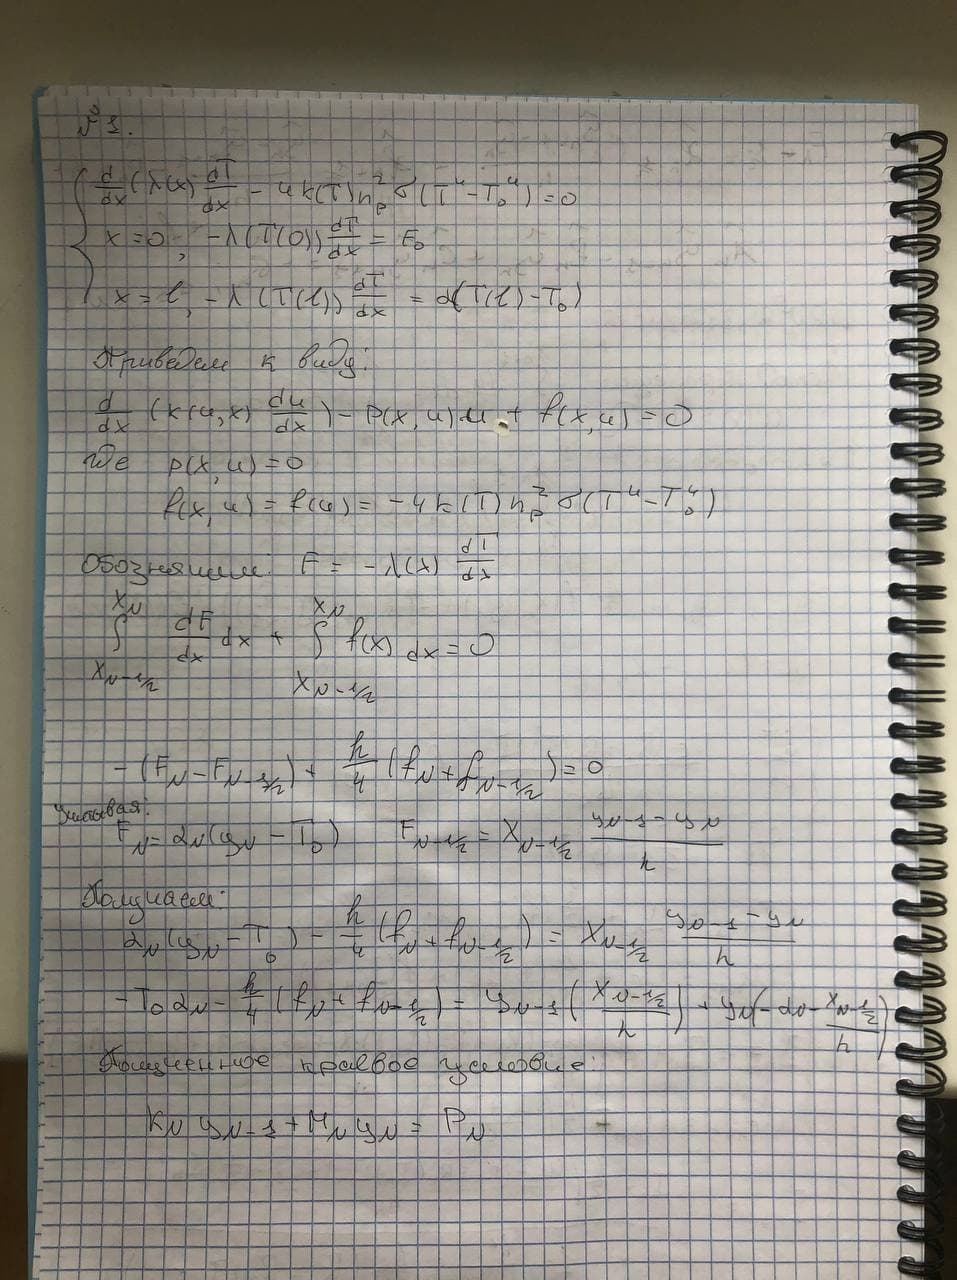
\includegraphics[width=0.8\textwidth]{img/task_1.jpg}}
\end{figure}


% Проинтегрируем уравнение на отрезке [$X_{n - \frac{1}{2}}; x_{n}$]

% \begin{equation*}
% 	- \int^{x_{n}}_{x_n - \frac{1}{2}} \frac{dF}{dx} dT - \int^{x_n}_{x_n - \frac{1}{2}} P(T) \cdot T^4 dT + \int^{x_{n}}_{x_{n} - \frac{1}{2}} f(t) dT = 0
% \end{equation*}

% Второй и третий интеграл вычислим с помощью метода трапеций:

% \begin{equation*}
% 	F_{n - \frac{1}{2}} - F_{n} - \frac{h}{4} (p_{n} y_{n} + p_{n - \frac{1}{2}}y_{n-\frac{1}{2}}) + \frac{h}{4} (f_{n} + f_{n - \frac{1}{2}}) = 0
% \end{equation*}

% Зная, что: 

% \begin{equation*}
% 	F_{n - \frac{1}{2}} = x_{n - \frac{1}{2}} \frac{y_{n - 1}}{y_n}{h}
% \end{equation*}

% \begin{equation*}
% 	F_{n} = \alpha_{n}(y_{n} - T_{0})
% \end{equation*}

% \begin{equation*}
% 	y_{n - \frac{1}{2}} = \frac{y_{n} + y_{n - 1}}{2h}
% \end{equation*}

% Имеем:

% \begin{equation*}
% 	\frac{x_{n - \frac{1}{2}} y_{n - 1}}{h} - \frac{x_{n - \frac{1}{2}}y_{n}}{h} - \alpha_{n}y_{n} + \alpha_{n} T_{0} - \frac{hp_{n}y_{n}}{48} - \frac{hp_{n - \frac{1}{2}}y_{n}}{8} - \frac{hp_{n - \frac{1}{2}}y_{n - 1}}{8} + \frac{f_{n - \frac{1}{2}} + f_{n}}{4}h = 0
% \end{equation*}

% \begin{equation*}
% 	y_{n}(-\frac{x_{n - \frac{1}{2}}}{h} - \alpha_{n} - \frac{hp_{n}}{4} - \frac{hp_{n} - \frac{1}{2}}{8}) + y_{n - 1}(\frac{x_{n - \frac{1}{2}}}{h} - \frac{hp_{n - \frac{1}{2}}}{8}) = -(\alpha_{n}T_{0} + \frac{f_{n} - \frac{1}{2}}{4}h)
% \end{equation*}

\clearpage

\subsection{2. График зависимости температуры $T(x)$ координаты $x$ при заданных выше параметрах.}
Выяснить, как сильно зависят результаты расчета T(x) и необходимое для
этого количество итераций от начального распределения температуры и шага сетки. 

\begin{figure}[ht!]
	\centering{
		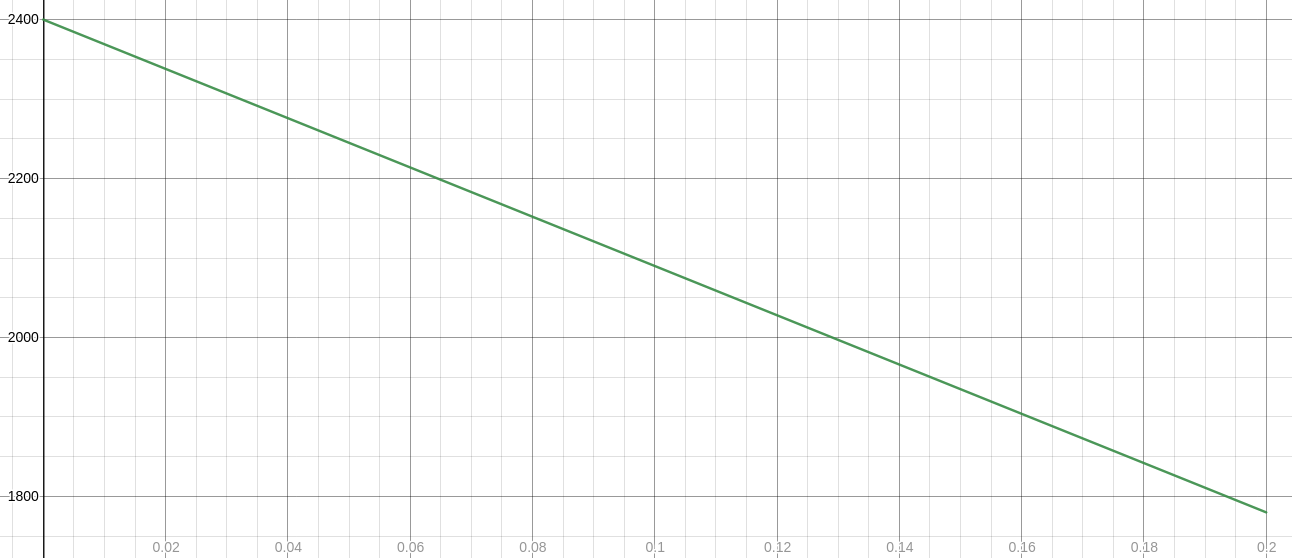
\includegraphics[width=0.6\textwidth]{img/1.png}}
\end{figure}
Кол-во итераций: 23

Изменим параметры: $T_0$ = 2000. 

\begin{figure}[ht!]
	\centering{
		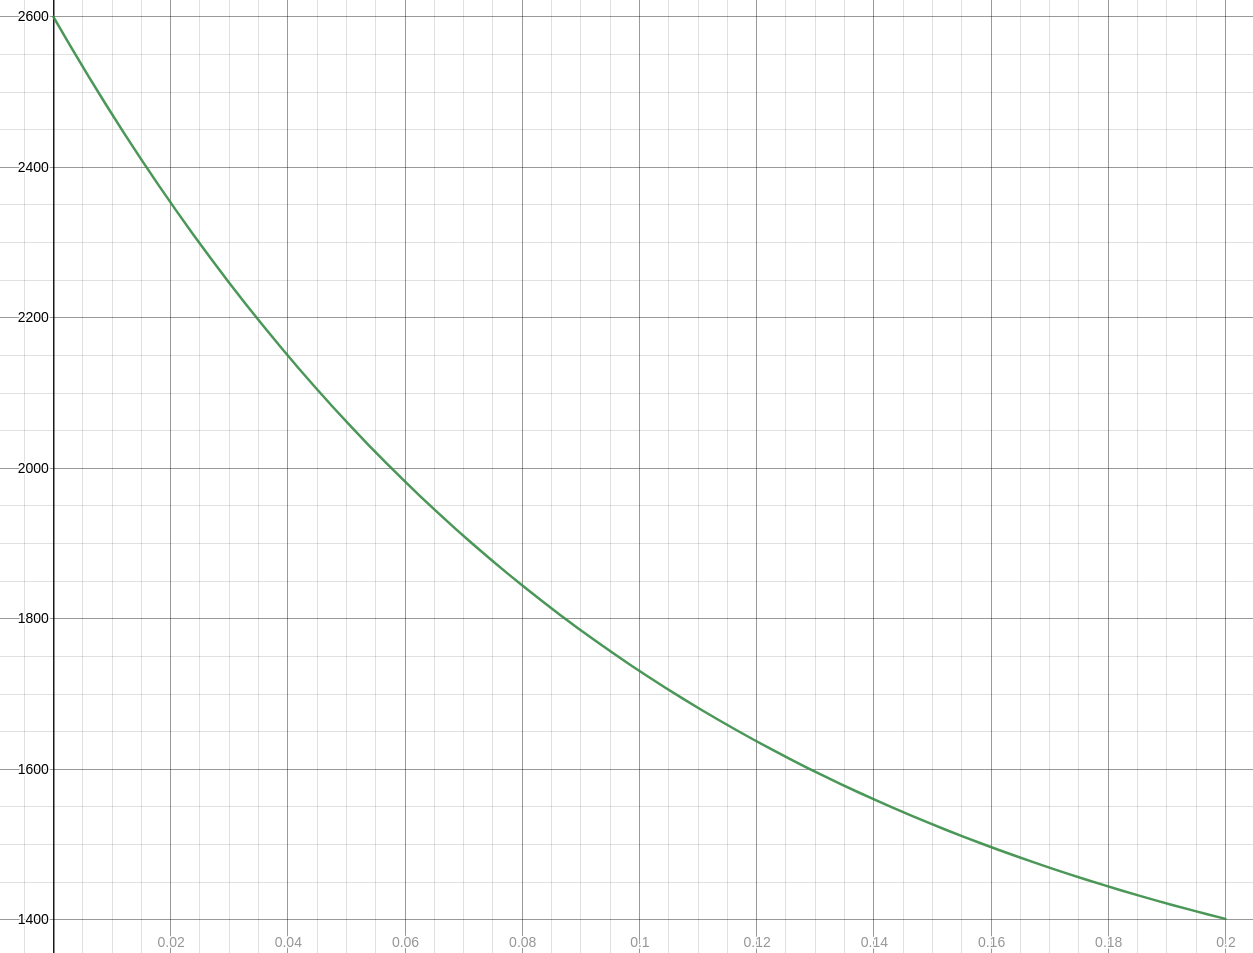
\includegraphics[width=0.6\textwidth]{img/2.png}}
\end{figure}
Кол-во итераций: 9

При увеличении $T_0$ получается более выраженная выпуклость кривых.
При этом количество итераций значительно снижается.

\newpage

\subsection{3. График зависимости $T(x)$ при $F_{0} = -10 \frac{Bт}{cm^2}$. }


\begin{figure}[ht!]
	\centering{
		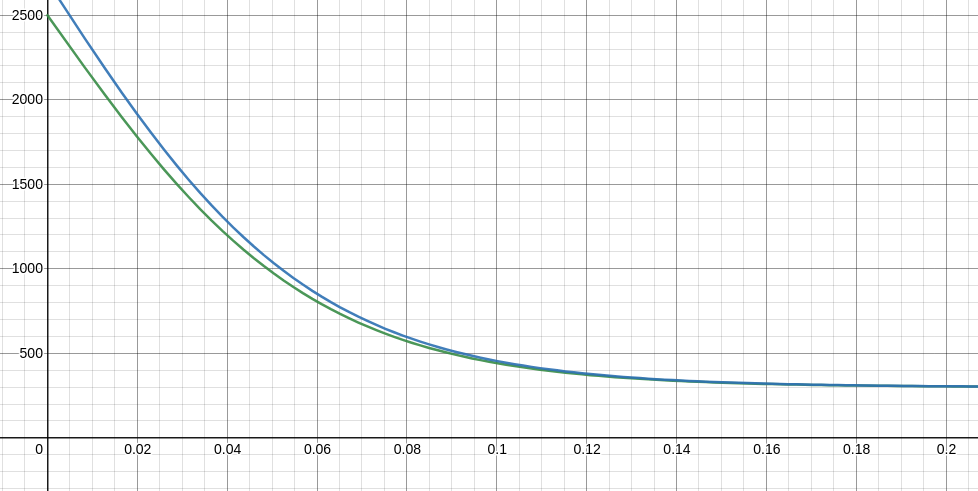
\includegraphics[width=0.6\textwidth]{img/3.png}}
\end{figure}

\newpage

\subsection{4. График зависимости $T(x)$ при увеличенных значениях $\alpha$ (например, в 3 раза). Сравнить с п. 2.}

Синяя кривая при увеличенном в 3 раза коэффициенте теплоотдачи.
\begin{figure}[ht!]
	\centering{
		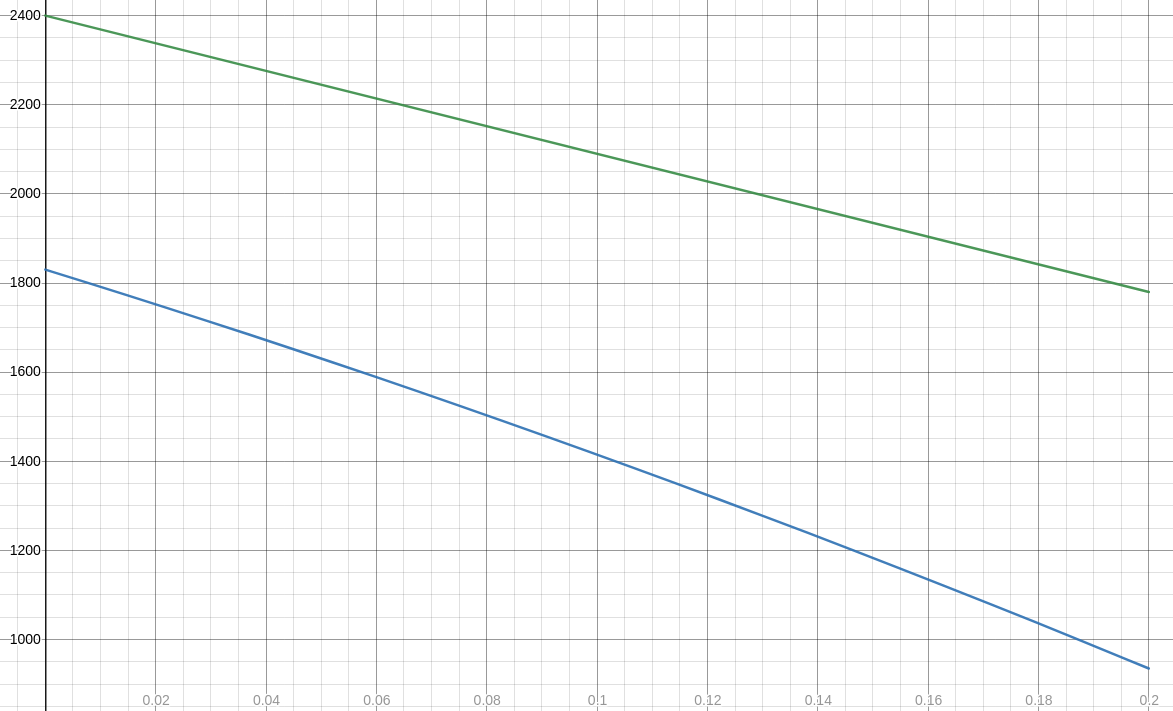
\includegraphics[width=0.6\textwidth]{img/4.png}}
\end{figure}

Зеленая кривая при увеличенном в 3 раза коэффициенте теплоотдачи.
\begin{figure}[ht!]
	\centering{
		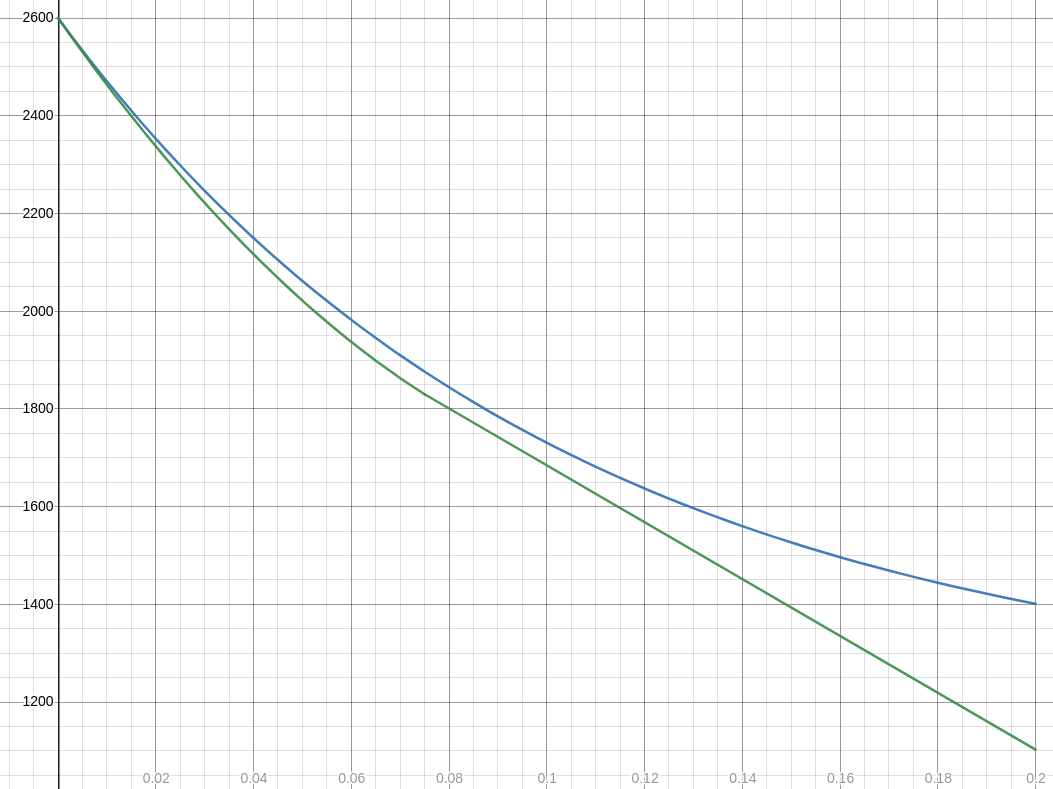
\includegraphics[width=0.6\textwidth]{img/5.png}}
\end{figure}

\newpage

\subsection{5. График зависимости $T(x)$ при $F_{0} = 0$.}

\begin{figure}[ht!]
	\centering{
		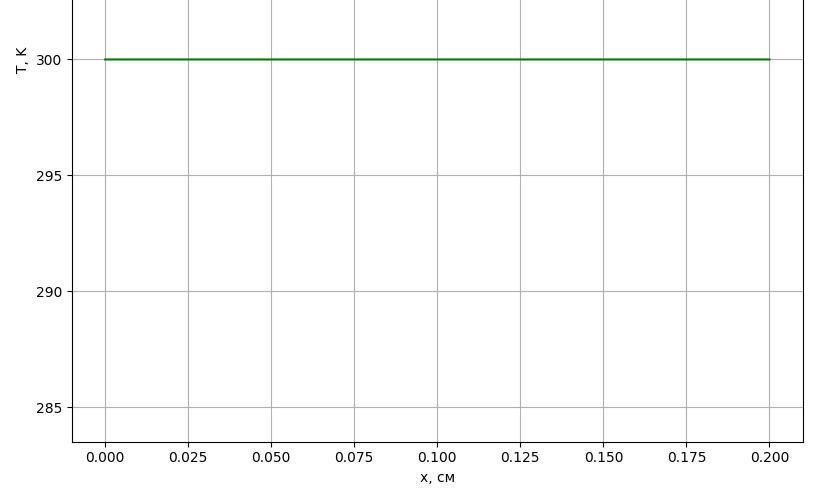
\includegraphics[width=0.6\textwidth]{img/6.png} }
\end{figure}

\subsection{6. Для указанного в задании исходного набора параметров привести данные по балансу энергии.}

\begin{itemize}
	\item Точность выхода $\varepsilon_{1} = $ 1e-5 (по температуре)
	\item Точность выхода $\varepsilon_{2} = $ 1e-3 (по балансу)
\end{itemize}


\newpage
\section{Ответы на вопросы}

\textbf{1. Какие способы тестирования программы можно предложить?}\\

В данной программе можно предложить тестирование при помощи изменения значения параметра 
$F_0$. Также при $F_0 > 0$ происходит охлаждение пластины, при $F_0 < 0$ нагревание. При увеличении теплосъема и неизменном потоке
$F_0$ уровень температур T(x) должен снижаться, а градиент увеличиваться.


\textbf{2. Получите  простейший разностный аналог нелинейного краевого условия при $x = l$.}\\

\begin{figure}[ht!]
	\centering{
		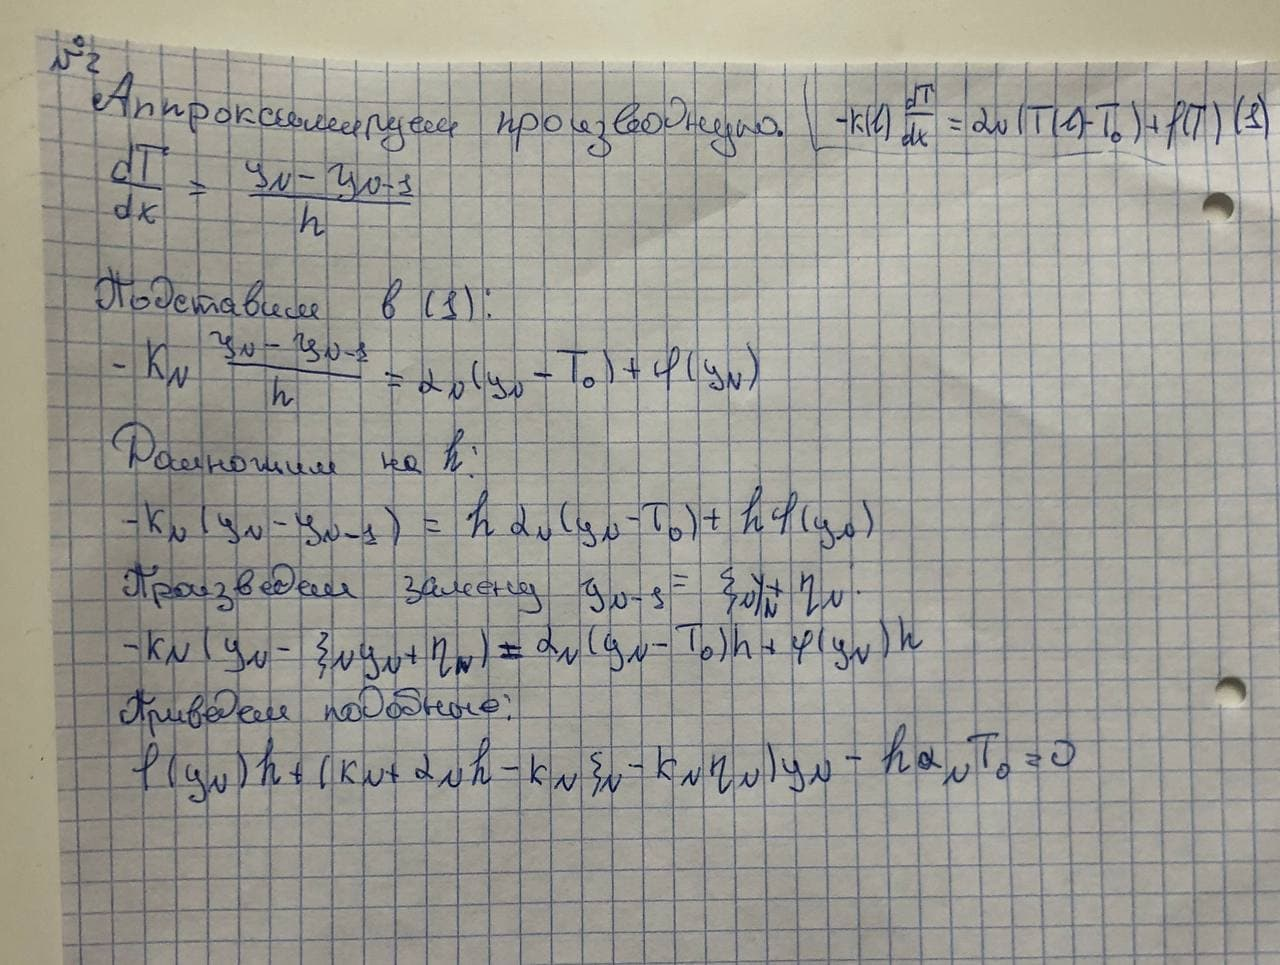
\includegraphics[width=0.7\textwidth]{img/v1.jpg}}
\end{figure}


\textbf{3. Опишите алгоритм применения метода прогонки, если при $x = 0$ краевое условие квазилинейное (как в настоящей работе), а при $x = l$, как в п. 2.}\\

\begin{figure}[ht!]
	\centering{
		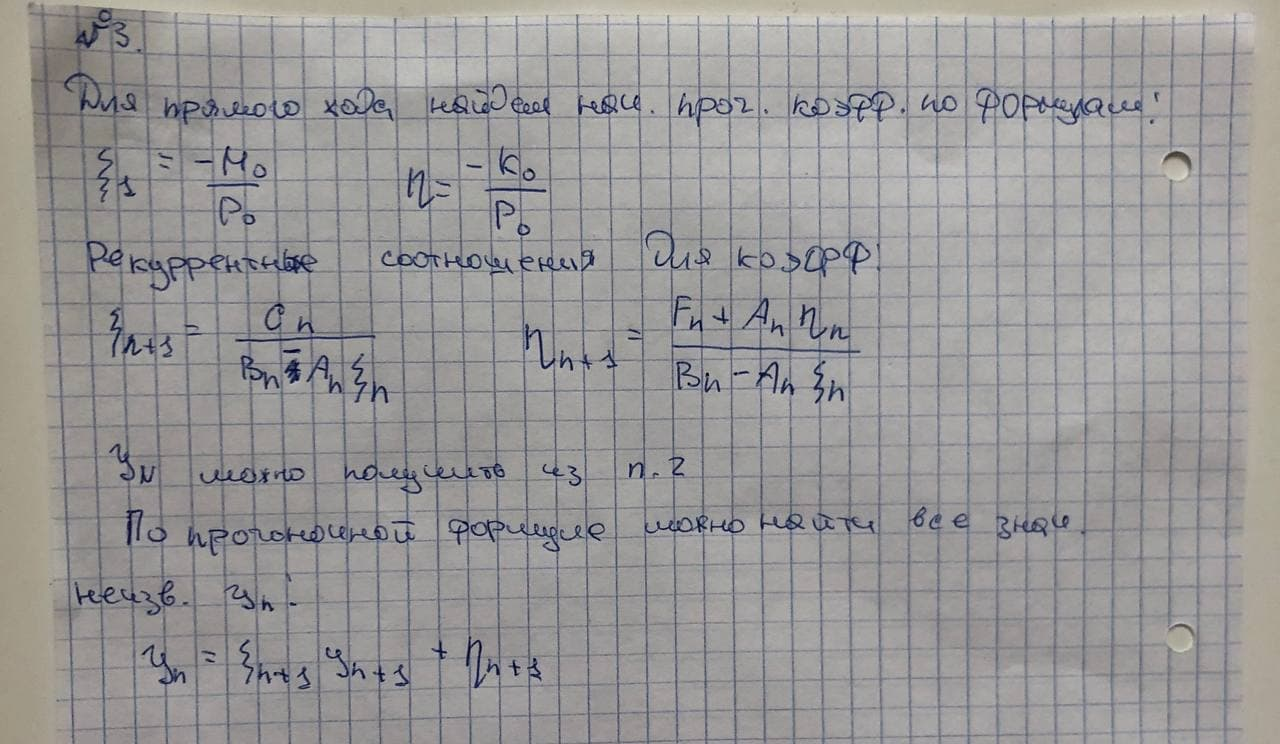
\includegraphics[width=0.7\textwidth]{img/v2.jpg}}
\end{figure}

\textbf{4. Опишите алгоритм определения единственного значения сеточной функции $y_p$ в одной заданной точке $p$. Использовать встречную прогонку, т.е. комбинацию правой и левой прогонок.}\\

\begin{figure}[ht!]
	\centering{
		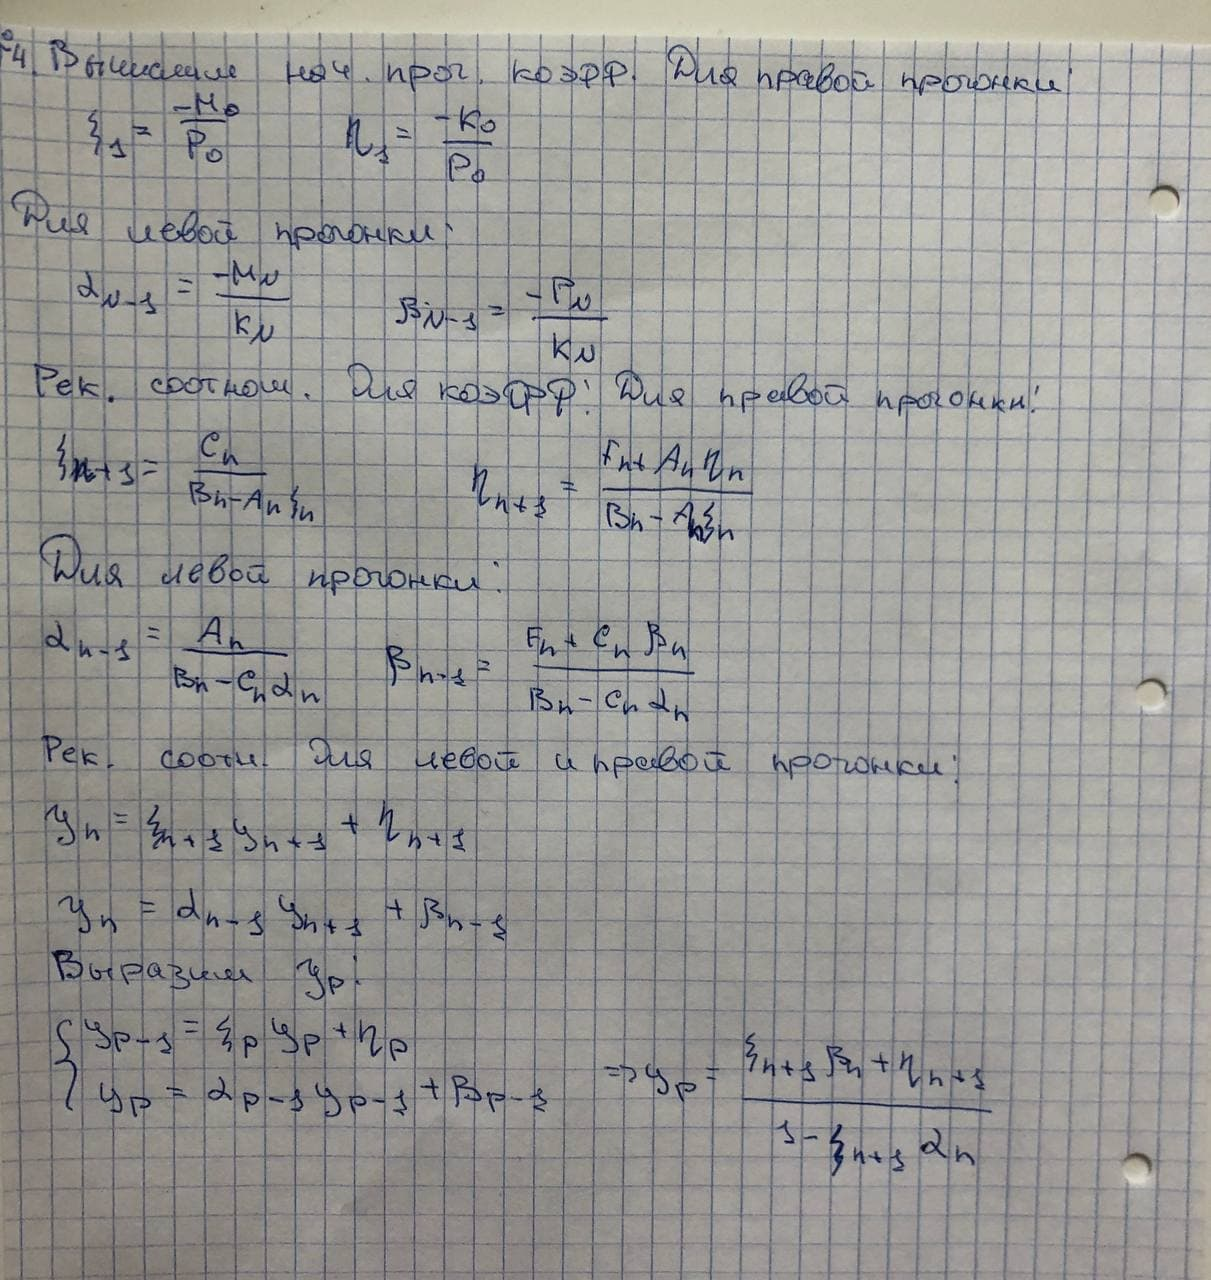
\includegraphics[width=0.7\textwidth]{img/v3.jpg}}
\end{figure}

\end{document}